\documentclass{beamer}
\usepackage[utf8]{inputenc}
\usepackage[spanish]{babel}
\usepackage{graphicx,hyperref,ru,url}

% The title of the presentation:
%  - first a short version which is visible at the bottom of each slide;
%  - second the full title shown on the title slide;
\title[Mathematical model on Alzheimer's disease]{
  Perspectives on mathematical modelling for Alhzeimer's disease}

% Optional: a subtitle to be dispalyed on the title slide
\subtitle{}

% The author(s) of the presentation:
%  - again first a short version to be displayed at the bottom;
%  - next the full list of authors, which may include contact information;
\author[Bartolomé Ortiz Viso]{
  Bartolomé Ortiz Viso \\\medskip
  {\small \url{bortiz@correo.ugr.es}} \\ 
  {\small \url{@bortizmath}}}

% The institute:
%  - to start the name of the university as displayed on the top of each slide
%    this can be adjusted such that you can also create a Dutch version
%  - next the institute information as displayed on the title slide
\institute[Universidad de Granada]{
  Dinámica celular y tumoral  \\
  Máster en Física y Matemáticas}

% Add a date and possibly the name of the event to the slides
%  - again first a short version to be shown at the bottom of each slide
%  - second the full date and event name for the title slide
\date[17 Enero, 2018]{
  17 Enero, 2018}

\begin{document}

\begin{frame}
  \titlepage
\end{frame}

\begin{frame}
  \frametitle{Índice}

  \tableofcontents
\end{frame}

\section{Introducción}

\begin{frame}
  \frametitle{Introducción}
\begin{columns}[t]
	\column{0.5\textwidth}
	La enfermedad de Alzheimer (DA, por sus siglas en inglés), es una \textbf{enfermedad neurodegenerativa}.
	
	 Se caracteriza en su forma típica por una pérdida de la memoria inmediata y de otras capacidades mentales en representacion directa de la muerte de las células nerviosas con la consiguiente atrofia cerebral.
	
	\column{0.5\textwidth}
	\begin{figure}[Atrofia cerebral]
		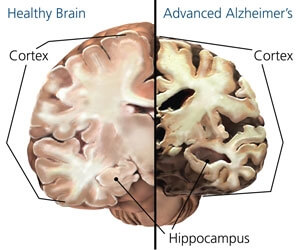
\includegraphics[scale=0.46]{alzheimer-cerebro-imagen.jpg}
		\caption{Representacion del deterioro cerebral}
		\label{cerebro}
	\end{figure}
\end{columns}
\end{frame}

\section{Mecanismos biológicos implicados}

\begin{frame}
  \frametitle{Mecanismos biológicos implicados}

  \begin{block}{A tener en cuenta}
    Aún no se conocen las causas exactas de la enfermedad, aunque se investigan varias hipótesis.
    El conocimiento actual, y los modelos, se basan en los marcadores patológicos que se sabe están implicados.
  \end{block}
  \begin{block}{Principales variables/componentes de los estudios}
    \begin{enumerate}
    	\item Poblaciones neuronales
    	\item Péptidos de Beta-Amiloide (C. priónico:A, Sin él:B)
    	\item Microglia
    	\item Astroglia
    	\item Proteinas $PPA$ y $PrP^C$
    	\item Escala temporal (microscópica: A, macroscópica: B)
    \end{enumerate}
      \end{block}
\end{frame}

\begin{frame}{Mecanismo biológicos implicados}
	\begin{figure}[Atrofia cerebral]
		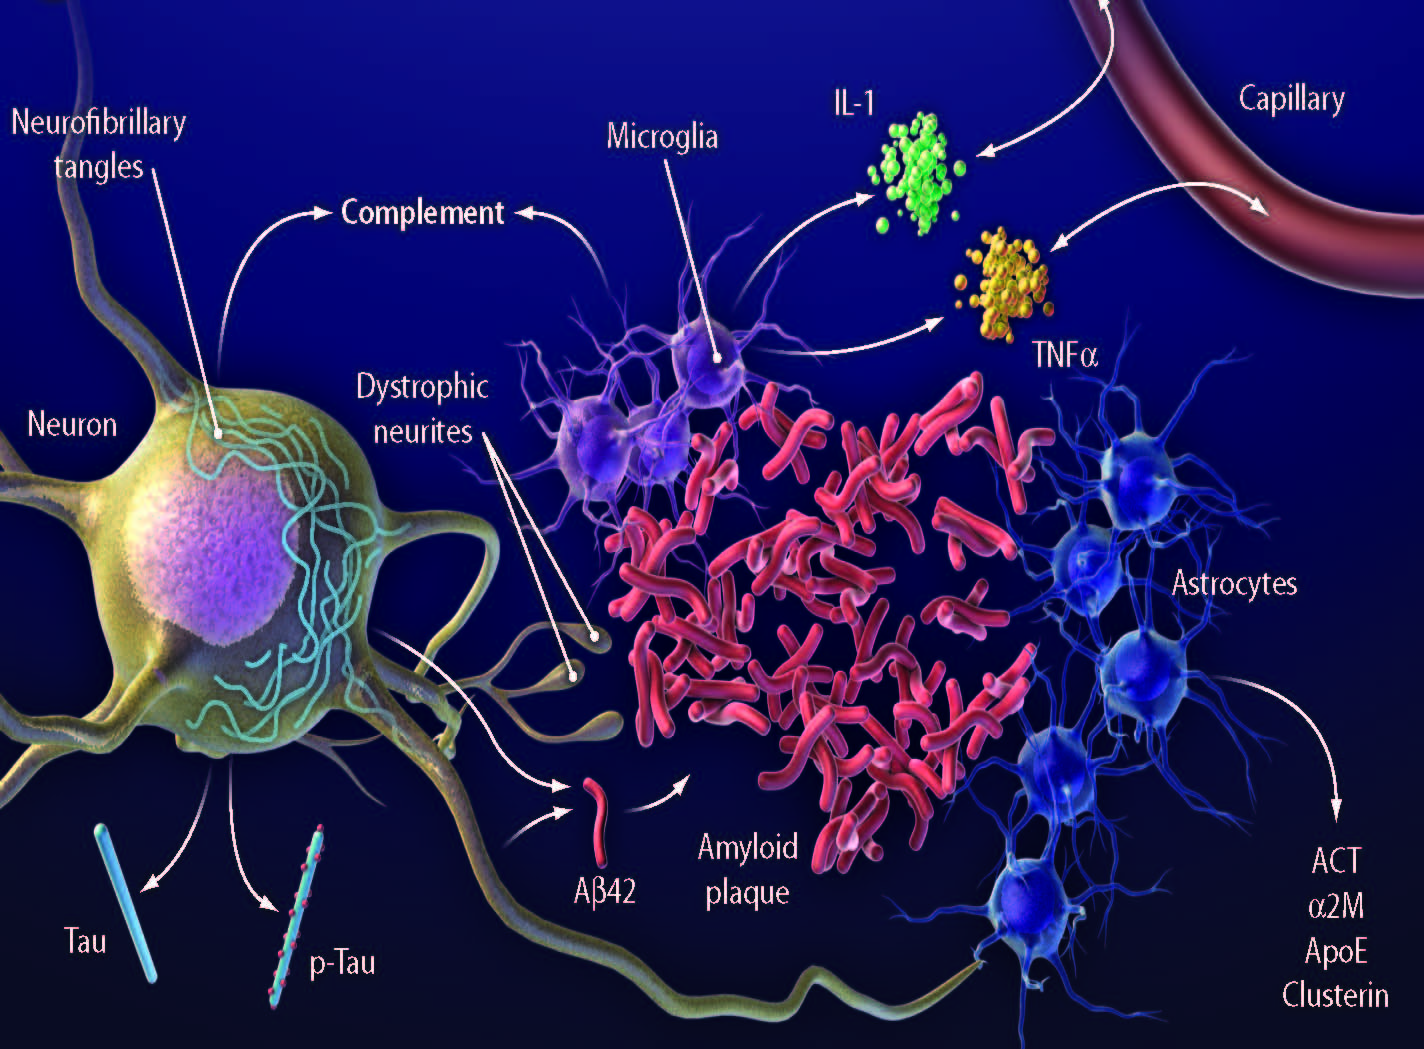
\includegraphics[scale=0.9]{imagen.jpg}
		\label{cerebro4}
	\end{figure}
\end{frame}


\section{Propuestas de modelado}

\subsection{Patogénesis}
\begin{frame}
  \frametitle{Resultados teóricos: 1º Modelo. 1,2B,3,4,6B}
\begin{block}{Puri, Ishwar K and Li, Liwu}
	Mathematical modeling for the pathogenesis of Alzheimer's disease
	\end{block}
	\begin{figure}[Esquema]
		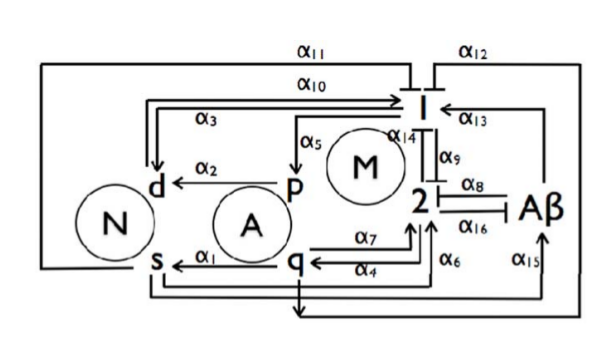
\includegraphics[scale=0.3]{primerdiagrama1.png}
		\caption{Representacion esquemática del mecanismo}
		\label{cerebro2}
	\end{figure}
\end{frame}

\begin{frame}
	\frametitle{Resultados teóricos: 1º Modelo. 1,2B,3,4,6B}
	\begin{equation}
	\left\lbrace
	\begin{array}{ll}
		dN_s/dt=\alpha_1A_q-\alpha_2A_p-\alpha_3M_1 \\
		dN_s/dt=-dN_d/dt\\
		dA_q/dt=\alpha_4M_2-\alpha_5M_1 \\
		-dA_q/dt=dA_p/dt \\
		dM_2/dt=(\alpha_6+\alpha_{11})N_s-\alpha_{10}N_d-(\alpha_7+\alpha_{12})A_q-\alpha_9M_1\\+\alpha_{14}M_2-(\alpha_8+\alpha_{13})A\beta\\
		dM_1/dt=-dM_2/dt \\
		dA\beta/dt=\alpha_{15}N_s-\alpha_{16}M
	\end{array}
	\right.
\end{equation}

\end{frame}

\begin{frame}
	\frametitle{Resultados teóricos: 1º Modelo. 1,2B,3,4,6B}
\begin{columns}[t]
	\column{0.5\textwidth}
	    \begin{enumerate}
	    	\item Estudio de la sensibilidad de parámetros
	    	\item Destacar el recorrido $M_2\longmapsto A\beta$
	    	\item ¿Eficacia de los tratamientos si removemos $A\beta$?
	    	\item Valores de $M_1 ,N_d, A\beta$ en la gráfica $\rightarrow$
	    \end{enumerate}
	
	\column{0.5\textwidth}
	\begin{figure}[Atrofia cerebral]
		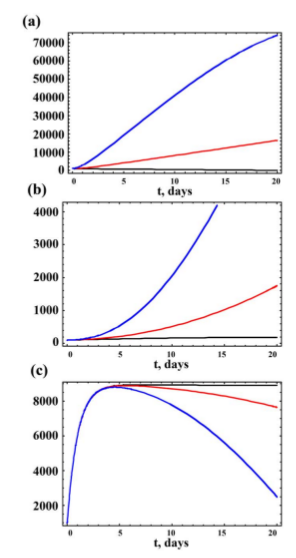
\includegraphics[scale=0.32]{primerAB.png}
		\caption{Valores de $M_1 ,N_d, A\beta$}
		\label{cerebro4}
	\end{figure}
\end{columns}
	
\end{frame}

\subsection{Incorporación de comportamiento priónico}
\begin{frame}
	\frametitle{Resultados teóricos: 2º Modelo. 1,2A,5,6A}
	\begin{block}{Helal, Mohamed and Hingant, Erwan and Pujo-Menjouet, Laurent and Webb, Glenn F.}
		Alzheimer’s disease: analysis of a mathematical model incorporating the role of prions
	\end{block}
	\begin{figure}[Esquema]
		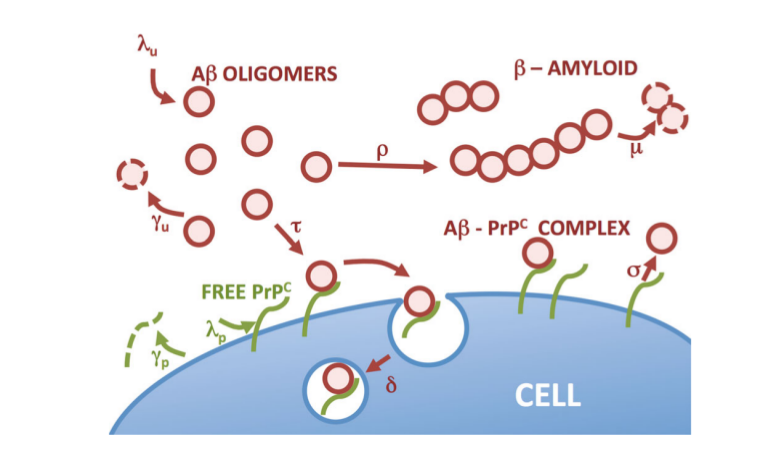
\includegraphics[scale=0.3]{segunda1.png}
		\caption{Representacion esquemática del mecanismo}
		\label{cerebro5}
	\end{figure}
\end{frame}

\begin{frame}
	\frametitle{Resultados teóricos: 2º Modelo. 1,2A,5,6A}
	
	\begin{enumerate}
		\item $f:=$Densidad de placa $\beta$-amiloide 
		\item $u(t)\geq0$ Concentración de $A\beta$ oligomeros
		\item $p(t)\geq0$ Concentración de $PrP^c$
		\item $p(t)\geq0$ Concentración de complejos $A\beta-x-PrP^c$ 
	\end{enumerate}
	\begin{equation}
	\left\lbrace
	\begin{array}{ll}
	\partial_tf(t,x)+u(t)\partial_x[\rho(x)f(t,x)]=\mu(x)f(x,t) \\
	du/dt=\lambda_u-\gamma_u-\tau u p+\sigma b-nN(u)-\frac{1}{3}u\int_{x_0}^{\infty}p(x)f(x,t)dx\\
	dp/dt=\lambda_p-\gamma_pp-\tau u p+\sigma b  \\
	db/dt=\tau u p-(\sigma+\delta)b
	\end{array}
	\right.
	\end{equation}
	
\end{frame}

\begin{frame}
	\frametitle{Resultados teóricos: 2º Modelo. 1,2A,5,6A}
	\begin{columns}[t]
		\column{0.5\textwidth}
		\begin{enumerate}
			\item La formación de polimeros es compleja e intervienen muchos procesos.
			\item No todo conjunto $A\beta$ es estable
			\item Diferentes tipos y constantes de polimerizacion
			\item El resultado teórico expone una estabilidad ¿Es representativo?
		\end{enumerate}
		
		\column{0.5\textwidth}
		\begin{figure}[Atrofia cerebral]
			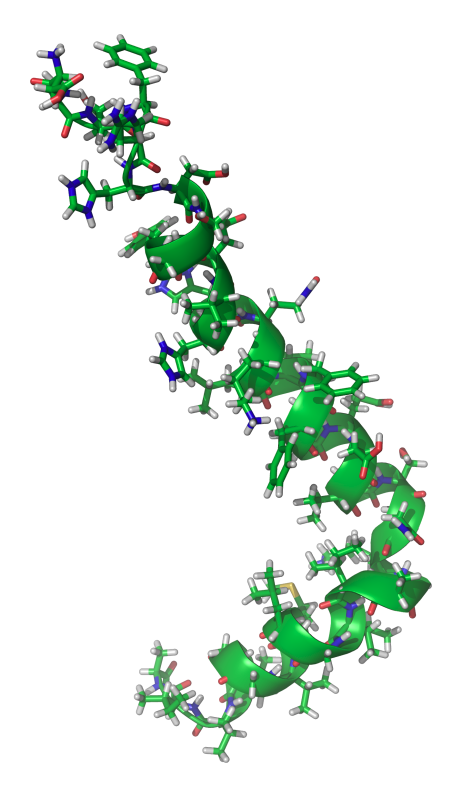
\includegraphics[scale=0.15]{beta.png}
			\caption{Molecula de $Amiloide\beta$}
			\label{cerebro4}
		\end{figure}
	\end{columns}
	
\end{frame}

\subsection{Comportamiento priónico +Difusión+Transporte}
\begin{frame}
	\frametitle{Resultados teóricos: 3º Modelo. 1,2A,5,6AB}
	\begin{block}{Bertsch, Michiel and Franchi, Bruno and Marcello, Norina and Tesi, Maria Carla and Tosin, Andrea}
		Alzheimer's disease: a mathematical model for onset and progression
	\end{block}
	2 escalas temporales: Una para la difusión:
	$$\partial_tu_m=d_m\nabla^2u_m+[\frac{1}{2}\sum_{j=1}^{m-1}a_{j,m}u_ju_{m-j}-u_m\sum_{j=1}^{N}a_{m,j}u_j]$$
	 otra para el progreso de la enfermedad:
	 $$\partial_tf+\partial_a(f\nu[f])=J[f]$$
\end{frame}

\begin{frame}
	\frametitle{Resultados teóricos: 3º Modelo. 1,2A,5,6AB}
	\begin{equation}
	\left\lbrace
	\begin{array}{ll}
	\partial_tf+\partial_a(f\nu[f])=J[f] \\
\epsilon\partial_tu_1=d_1\nabla^2u_1+[u_1\sum_{j=1}^{N}a_{1,j}u_j]+F[f]-\sigma_1u_1\\
	\epsilon\partial_tu_m=d_m\nabla^2u_m+[\frac{1}{2}\sum_{j=1}^{m-1}a_{j,m}u_ju_{m-j}-u_m\sum_{j=1}^{N}a_{m,j}u_j]  \\
	\epsilon\partial_tu_N=+\frac{1}{2}\sum_{j+k\geq N}a_{j,k}u_ju_k
	\end{array}
	\right.
	\end{equation}
	
\end{frame}

\begin{frame}
	\frametitle{Resultados numéricos: 3º Modelo. 1,2A,5,6AB}

		\begin{figure}[Atrofia cerebral]
			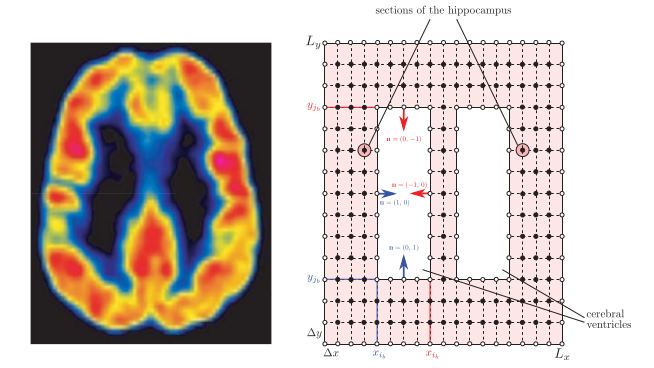
\includegraphics[scale=0.4]{tercer1.png}
			\caption{Esquema de simulación numérica}
			\label{cerebro4}
		\end{figure}

	
\end{frame}
\begin{frame}
	\frametitle{Resultados numéricos: 3º Modelo. 1,2A,5,6AB}
	
	\begin{figure}[Atrofia cerebral]
		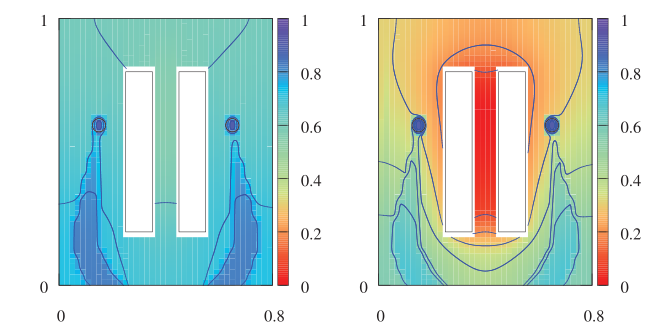
\includegraphics[scale=0.4]{tercer2.png}
		\caption{Expansión de malfuncionamiento neuronal}
		\label{cerebro4}
	\end{figure}
	
	
\end{frame}
\begin{frame}
	\frametitle{Resultados numéricos: 3º Modelo. 1,2A,5,6AB}
	
	\begin{figure}[Atrofia cerebral]
		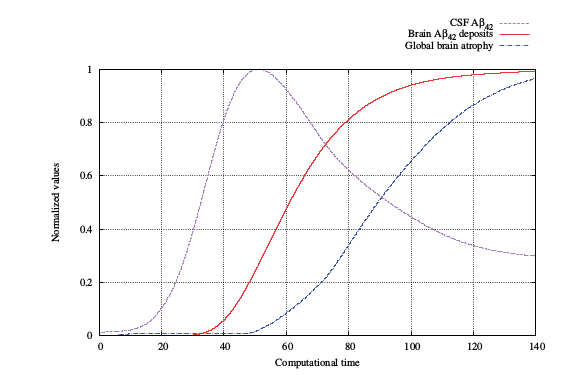
\includegraphics[scale=0.4]{tercer3.png}
		\caption{Evolución de los biomarcadores}
		\label{cerebro4}
	\end{figure}
	
	
\end{frame}



\subsection{Comportamiento global}
\begin{frame}
	\frametitle{Resultados teóricos: 4º Modelo. 1,2A,3,4,5,6B}
	\begin{block}{Hao, Wenrui and Friedman, Avner}
		Mathematical model on Alzheimer’s disease
	\end{block}
	Pretende presentar un modelo amplio y completo para la identificación de posibles vías para mitigar la enfermedad. Tratamiento analítico se hace inviable debido a la cantidad de ecuaciones que se presentan.
\end{frame}

\begin{frame}
	\frametitle{Resultados teóricos: 4º Modelo. 1,2A,3,4,5,6B}
	
	\begin{figure}[Atrofia cerebral]
		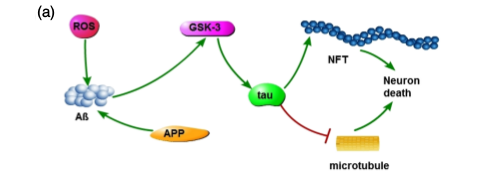
\includegraphics[scale=0.6]{primerdiagrama.png}
		\caption{Evolución del sistema biológico}
		\label{cerebro4}
	\end{figure}
	
\end{frame}

\begin{frame}
	\frametitle{Resultados teóricos: 4º Modelo. 1,2A,3,4,5,6B}
	\begin{figure}[Atrofia cerebral]
		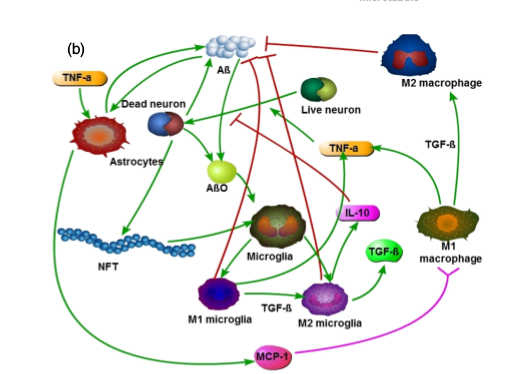
\includegraphics[scale=0.4]{segundodiagrama.png}
		\caption{Evolución del sistema biológico}
		\label{cerebro4}
	\end{figure}
	
\end{frame}

\begin{frame}
	\frametitle{Resultados teóricos: 4º Modelo. 1,2A,3,4,5,6B}
	\begin{figure}[Atrofia cerebral]
		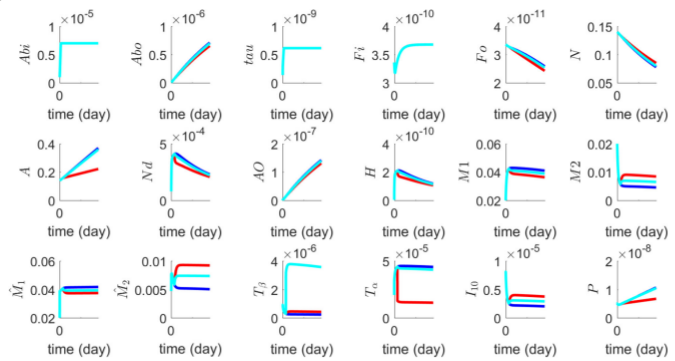
\includegraphics[scale=0.4]{cuarto.png}
		\caption{Evolución del sistema con tratamiento o sin el}
		\label{cerebro4}
	\end{figure}
	
\end{frame}
\begin{frame}
	\frametitle{Resultados teóricos: 4º Modelo. 1,2A,3,4,5,6B}
	\begin{figure}[Atrofia cerebral]
		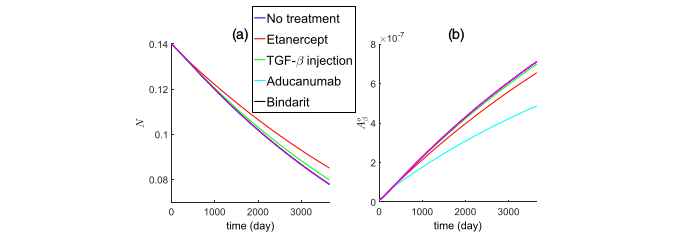
\includegraphics[scale=0.4]{quinto.png}
		\caption{Evolucion de la enfermedad con distintos tratamientos}
		\label{cerebro4}
	\end{figure}
	
\end{frame}

\begin{frame}
	\frametitle{Resultados teóricos: 4º Modelo. 1,2A,3,4,5,6B}
	\begin{figure}[Atrofia cerebral]
		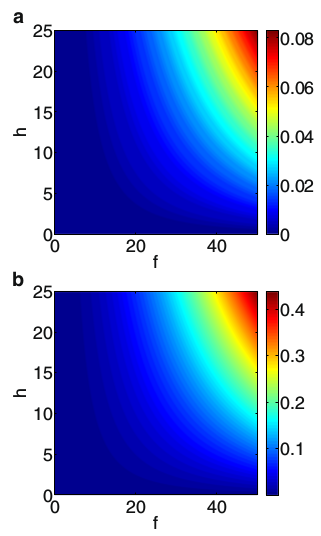
\includegraphics[scale=0.25]{sexta.png}
		\caption{Efectividad del tratamiento con la simulación}
		\label{cerebro4}
	\end{figure}
	
\end{frame}



\section{Conclusiones y futuro trabajo}

\begin{frame}
	\frametitle{Conclusiones y futuro trabajo}
	
	\begin{itemize}
		\item Problema de gran complejidad
		\item Fuente de nuevas matemáticas
		\item Desarrollo de simulaciones 
		\item Importancia de completmentar desarrollo teórico y numérico
		\item Importancia de la interdisciplinariedad
	\end{itemize}
\end{frame}

\end{document}